\documentclass{article}

\usepackage{fancyhdr}
\usepackage{extramarks}
\usepackage{amsmath}
\usepackage{amsthm}
\usepackage{amsfonts}
\usepackage{amssymb,booktabs,array,needspace}
\usepackage{tikz}
\usepackage[plain]{algorithm}
\usepackage{algpseudocode}
\usepackage{enumerate}
\usepackage{hyperref}
\usetikzlibrary{automata,positioning}

%
% Basic Document Settings
%  
                    
\topmargin=-0.45in
\evensidemargin=0in
\oddsidemargin=0in
\textwidth=6.5in
\textheight=9.0in
\headsep=0.25in

\linespread{1.1}

\pagestyle{fancy}
\lhead{\hmwkAuthorName}
\chead{\hmwkClass : \hmwkTitle}
\rhead{\firstxmark}
\lfoot{\lastxmark}
\cfoot{\thepage}

\renewcommand\headrulewidth{0.4pt}
\renewcommand\footrulewidth{0.4pt}

\setlength\parindent{0pt}

%
% Create Problem Sections
%

\newcommand{\enterProblemHeader}[1]{
    \nobreak\extramarks{}{Problem \arabic{#1} continued on next page\ldots}\nobreak{}
    \nobreak\extramarks{Problem \arabic{#1} (continued)}{Problem \arabic{#1} continued on next page\ldots}\nobreak{}
}

\newcommand{\exitProblemHeader}[1]{
    \nobreak\extramarks{Problem \arabic{#1} (continued)}{Problem \arabic{#1} continued on next page\ldots}\nobreak{}
    \stepcounter{#1}
    \nobreak\extramarks{Problem \arabic{#1}}{}\nobreak{}
}

\newcommand*\circled[1]{\tikz[baseline=(char.base)]{
		\node[shape=circle,draw,inner sep=2pt] (char) {#1};}}


\setcounter{secnumdepth}{0}
\newcounter{partCounter}
\newcounter{homeworkProblemCounter}
\setcounter{homeworkProblemCounter}{1}

%
% Homework Problem Environment
%
% This environment takes an optional argument. When given, it will adjust the
% problem counter. This is useful for when the problems given for your
% assignment is not sequential.
%

\newenvironment{homeworkProblem}[1][-1]{
    \ifnum#1>0
        \setcounter{homeworkProblemCounter}{#1}
    \fi
    \section{Problem \arabic{homeworkProblemCounter}}
    \setcounter{partCounter}{1}
    \enterProblemHeader{homeworkProblemCounter}
}{
    \exitProblemHeader{homeworkProblemCounter}
}

%
% Homework Details
%   - Title
%   - Class
%   - Due date
%   - Name
%   - Student ID

\newcommand{\hmwkTitle}{Homework 1}
\newcommand{\hmwkClass}{SI252 Reinforcement Learning}
\newcommand{\hmwkDueDate}{September 30, 2026}
\newcommand{\hmwkAuthorName}{jiang ye}
\newcommand{\hmwkAuthorID}{2026133019}


%
% Title Page
%

\title{
    \vspace{2in}
    \textmd{\textbf{\hmwkClass:\\  \hmwkTitle}}\\
    \normalsize\vspace{0.1in}\small{Due\ on\ \hmwkDueDate\ at 22:59}\\
	\vspace{4in}
}

\author{
	Name: \textbf{\hmwkAuthorName} \\
	Student ID: \hmwkAuthorID}
\date{}

\renewcommand{\part}[1]{\textbf{\large Part \Alph{partCounter}}\stepcounter{partCounter}\\}

%
% Various Helper Commands
%

% Useful for algorithms
\newcommand{\alg}[1]{\textsc{\bfseries \footnotesize #1}}
% For derivatives
\newcommand{\deriv}[1]{\frac{\mathrm{d}}{\mathrm{d}x} (#1)}
% For partial derivatives
\newcommand{\pderiv}[2]{\frac{\partial}{\partial #1} (#2)}
% Integral dx
\newcommand{\dx}{\mathrm{d}x}
% Alias for the Solution section header
\newcommand{\solution}{\par\medskip\noindent\textbf{\large Solution}\par\smallskip}
% Probability commands: Expectation, Variance, Covariance, Bias
\newcommand{\E}{\mathrm{E}}
\newcommand{\Var}{\mathrm{Var}}
\newcommand{\Cov}{\mathrm{Cov}}
\newcommand{\Bias}{\mathrm{Bias}}


% Layout and helper commands.
\setlength{\headheight}{14pt}
\setlength{\emergencystretch}{2em}
\hypersetup{hidelinks}
\newcommand{\PP}{\mathbb{P}}
\newcommand{\RR}{\mathbb{R}}
\newcommand{\ind}{\mathbf{1}}
\newcommand{\subpart}[1]{\par\medskip\Needspace{5\baselineskip}\textbf{#1}\par\smallskip}

\begin{document}

\hypersetup{pageanchor=false}
\maketitle
\thispagestyle{empty}
\clearpage
\setcounter{page}{1}
\hypersetup{pageanchor=true}

\begin{homeworkProblem}

    \solution 
    The motivation to introduce random variable is to map each sample point of a random experiment to a real number.
    This helps us to study its distribution, expectation, variance, and correlation.
    It is called a random variable rather than a random function because the correspondence rule of the function is fixed; however, the sample outcome ($\omega$) that actually occurs is random, so the function value ($X(\omega)$) is also random.
    Therefore, I believe the term "random variable" better emphasizes that the numerical quantity it maps changes as the outcome of the random experiment changes.

\end{homeworkProblem}

\begin{homeworkProblem}

    \solution
    \subpart{(a)}
    For X, Y both discrete:
    \[ p_{X,Y}(x,y)=\PP(Y=y\mid X=x)\PP(X=x) \]
    \[ p_{X,Y}(x,y)=\PP(X=x\mid Y=y)\PP(Y=y) \]
    Setting the two equations above equal, we obtain:
    \[ \PP(Y=y\mid X=x)=\frac{\PP(X=x\mid Y=y)\PP(Y=y)}{\PP(X=x)} \]
    For X is discrete and Y is continuous:
    \[ p_{X,Y}(x,y)=\PP(X=x)f_Y(y\mid X=x) \]
    \[ p_{X,Y}(x,y)=\PP(X=x\mid Y=y)f_Y(y) \]
    Setting the two equations above equal, we obtain:
    \[ f_Y(y\mid X=x)=\frac{\PP(X=x\mid Y=y)f_Y(y)}{\PP(X=x)} \]
    For Y is discrete and X is continuous:
    \[ p_{X,Y}(x,y)=\PP(Y=y)f_X(x\mid Y=y) \]
    \[ p_{X,Y}(x,y)=\PP(Y=y\mid X=x)f_X(x) \]
    Setting the two equations above equal, we obtain:
    \[ \PP(Y=y\mid X=x)=\frac{\PP(Y=y)f_X(x\mid Y=y)}{f_X(x)} \]
    For X, Y both continuous:
    \[ f_{X,Y}(x,y)=f_{Y\mid X}(y\mid x)f_X(x)=f_{X\mid Y}(x\mid y)f_Y(y) \]
    So we obtain:
    \[ f_{Y\mid X}(y\mid x)=\frac{f_{X\mid Y}(x\mid y)f_Y(y)}{f_X(x)} \]

    \subpart{(b)}
    For X, Y both discrete:
    \[ p_{X,Y}(x,y)=\PP(X=x\mid Y=y)\PP(Y=y) \]
    Summing over all possible values of Y, we obtain:
    \[ \PP(X=x)=\sum_y p_{X,Y}(x,y)=\sum_y \PP(X=x\mid Y=y)\PP(Y=y) \]
    For X is discrete and Y is continuous:
    \[ p_{X,Y}(x,y)=\PP(X=x\mid Y=y)f_Y(y) \]
    Integrating over all possible values of Y, we obtain:
    \[ \PP(X=x)=\int_{-\infty}^{\infty}p_{X,Y}(x,y)\,dy=\int_{-\infty}^{\infty}\PP(X=x\mid Y=y)f_Y(y)\,dy \]
    For Y is discrete and X is continuous:
    \[ p_{X,Y}(x,y)=f_X(x\mid Y=y)\PP(Y=y) \]
    Summing over all possible values of Y, we obtain:
    \[ f_X(x)=\sum_y p_{X,Y}(x,y)=\sum_y f_X(x\mid Y=y)\PP(Y=y) \]
    For X, Y both continuous:
    \[ f_{X,Y}(x,y)=f_{X\mid Y}(x\mid y)f_Y(y) \]
    Integrating over all possible values of Y, we obtain:
    \[ f_X(x)=\int_{-\infty}^{\infty}f_{X,Y}(x,y)\,dy=\int_{-\infty}^{\infty}f_{X\mid Y}(x\mid y)f_Y(y)\,dy \]

    \subpart{(c)}
    By the definition of conditional variance:
    \[ \Var(Y\mid X)=\E[Y^2\mid X]-(\E[Y\mid X])^2 \]
    Taking expectations and using the law of total expectation, we obtain:
    \[ \E[\Var(Y\mid X)]=\E[Y^2]-\E[(\E[Y\mid X])^2] \]
    Similarly, by the definition of variance:
    \[ \Var(\E[Y\mid X])=\E[(\E[Y\mid X])^2]-(\E[\E[Y\mid X]])^2 \]
    Since $\E[\E[Y\mid X]]=\E[Y]$, we obtain:
    \[ \Var(\E[Y\mid X])=\E[(\E[Y\mid X])^2]-(\E[Y])^2 \]
    Adding the two expressions, we obtain:
    \[ \E[\Var(Y\mid X)]+\Var(\E[Y\mid X])=\E[Y^2]-(\E[Y])^2=\Var(Y) \]

    \subpart{(d)}
    Assume X and Y have finite second moments and $\Var(X)>0$. Let:
    \[ \mu_X=\E[X],\qquad \mu_Y=\E[Y],\qquad \sigma_X^2=\Var(X),\qquad \sigma_Y^2=\Var(Y) \]
    We need to find a and b that minimize:
    \[ J(a,b)=\E[(Y-a-bX)^2] \]
    Writing the error in terms of centered random variables, we obtain:
    \[ Y-a-bX=(Y-\mu_Y)-b(X-\mu_X)+(\mu_Y-a-b\mu_X) \]
    Let $c=\mu_Y-a-b\mu_X$, which is a constant for fixed a and b. First, expanding the square gives:
    \[
    \begin{aligned}
        (Y-a-bX)^2
        &=(Y-\mu_Y)^2+b^2(X-\mu_X)^2+c^2 \\
        &\quad-2b(Y-\mu_Y)(X-\mu_X) \\
        &\quad+2c(Y-\mu_Y)-2bc(X-\mu_X).
    \end{aligned}
    \]
    Taking expectations term by term and moving constants outside the expectations, we obtain:
    \[
    \begin{aligned}
        J(a,b)
        &=\E[(Y-\mu_Y)^2]+b^2\E[(X-\mu_X)^2]+c^2 \\
        &\quad-2b\E[(Y-\mu_Y)(X-\mu_X)] \\
        &\quad+2c\E[Y-\mu_Y]-2bc\E[X-\mu_X].
    \end{aligned}
    \]
    Since $\mu_Y=\E[Y]$ and $\mu_X=\E[X]$, we have:
    \[ \E[Y-\mu_Y]=\E[Y]-\mu_Y=0,\qquad \E[X-\mu_X]=\E[X]-\mu_X=0 \]
    Therefore, the last two terms vanish. By the definitions of variance and covariance:
    \[ \E[(Y-\mu_Y)^2]=\Var(Y)=\sigma_Y^2,\qquad \E[(X-\mu_X)^2]=\Var(X)=\sigma_X^2 \]
    \[ \E[(Y-\mu_Y)(X-\mu_X)]=\Cov(X,Y) \]
    The product term is the covariance and does not vanish in general. Substituting these expressions and $c=\mu_Y-a-b\mu_X$, we obtain:
    \[ J(a,b)=\sigma_Y^2-2b\Cov(X,Y)+b^2\sigma_X^2+(\mu_Y-a-b\mu_X)^2 \]
    For any fixed b, the last term is minimized by choosing:
    \[ a=\mu_Y-b\mu_X \]
    Substituting this value makes the last term zero:
    \[ (\mu_Y-a-b\mu_X)^2=(\mu_Y-(\mu_Y-b\mu_X)-b\mu_X)^2=0 \]
    Therefore:
    \[ J(\mu_Y-b\mu_X,b)=\sigma_Y^2+b^2\sigma_X^2-2b\Cov(X,Y) \]
    To complete the square in b, first factor out $\sigma_X^2$ from the terms involving b:
    \[ b^2\sigma_X^2-2b\Cov(X,Y)=\sigma_X^2\left(b^2-2b\frac{\Cov(X,Y)}{\sigma_X^2}\right) \]
    Inside the parentheses, add and subtract the same squared quantity:
    \[
    \begin{aligned}
        b^2-2b\frac{\Cov(X,Y)}{\sigma_X^2}
        &=b^2-2b\frac{\Cov(X,Y)}{\sigma_X^2}
        +\left(\frac{\Cov(X,Y)}{\sigma_X^2}\right)^2
        -\left(\frac{\Cov(X,Y)}{\sigma_X^2}\right)^2 \\
        &=\left(b-\frac{\Cov(X,Y)}{\sigma_X^2}\right)^2
        -\left(\frac{\Cov(X,Y)}{\sigma_X^2}\right)^2.
    \end{aligned}
    \]
    Multiplying by $\sigma_X^2$, we obtain:
    \[ b^2\sigma_X^2-2b\Cov(X,Y)=\sigma_X^2\left(b-\frac{\Cov(X,Y)}{\sigma_X^2}\right)^2-\frac{\Cov(X,Y)^2}{\sigma_X^2} \]
    Adding back $\sigma_Y^2$, we obtain:
    \[ J(\mu_Y-b\mu_X,b)=\sigma_X^2\left(b-\frac{\Cov(X,Y)}{\sigma_X^2}\right)^2+\sigma_Y^2-\frac{\Cov(X,Y)^2}{\sigma_X^2} \]
    The last two terms do not depend on b, so only the squared term needs to be minimized.
    Since $\sigma_X^2>0$, the minimum is attained at:
    \[ b^*=\frac{\Cov(X,Y)}{\Var(X)},\qquad a^*=\E[Y]-b^*\E[X] \]
    So we obtain:
    \[ L[Y\mid X]=a^*+b^*X=\E[Y]+\frac{\Cov(X,Y)}{\Var(X)}(X-\E[X]) \]
    If $\Var(X)=0$, X is constant almost surely, and the optimal estimate is the constant $\E[Y]$.

    \subpart{(e)}
    Let $m(X)=\E[Y\mid X]$. By the definition of conditional expectation:
    \[ \E[Y-m(X)\mid X]=\E[Y\mid X]-m(X)=0 \]
    For any measurable function $\phi$ for which the following expectations are finite, $\phi(X)$ is determined by X. Therefore:
    \[ \E[(Y-m(X))\phi(X)\mid X]=\phi(X)\E[Y-m(X)\mid X]=0 \]
    Taking expectations, we obtain:
    \[ \E[(Y-\E[Y\mid X])\phi(X)]=0 \]
    Conversely, suppose $g(X)$ has a finite second moment and satisfies:
    \[ \E[(Y-g(X))\phi(X)]=0,\qquad \text{for every admissible }\phi \]
    Assume Y also has a finite second moment. Taking $\phi(X)=g(X)-m(X)$, we obtain:
    \[ \E[(Y-g(X))(g(X)-m(X))]=0 \]
    By the orthogonality property proved above, we also have:
    \[ \E[(Y-m(X))(g(X)-m(X))]=0 \]
    Subtracting the first equation from the second and using linearity of expectation, we obtain:
    \[
    \begin{aligned}
        0
        &=\E[(Y-m(X))(g(X)-m(X))]-\E[(Y-g(X))(g(X)-m(X))] \\
        &=\E[\bigl((Y-m(X))-(Y-g(X))\bigr)(g(X)-m(X))] \\
        &=\E[(g(X)-m(X))^2].
    \end{aligned}
    \]
    Here $(Y-m(X))-(Y-g(X))=g(X)-m(X)$.
    Since the squared term is nonnegative, we obtain:
    \[ g(X)=m(X)=\E[Y\mid X]\qquad\text{almost surely} \]

    \subpart{(f)}
    Let $W=Z-\E[Z]$. Then:
    \[ \E[W]=0,\qquad \E[W^2]=\sigma^2 \]
    For any constant $s\geq0$, the event $W\geq a$ implies $(W+s)^2\geq(a+s)^2$. By Markov's inequality:
    \[ \PP(W\geq a)\leq \PP((W+s)^2\geq(a+s)^2)\leq\frac{\E[(W+s)^2]}{(a+s)^2} \]
    Since $\E[W]=0$, we obtain:
    \[ \PP(W\geq a)\leq\frac{\E[(W+s)^2]}{(a+s)^2}=\frac{\E[W^2]+2sE(W)+s^2}{(a+s)^2}=\frac{\sigma^2+s^2}{(a+s)^2} \]
    Choosing $s=\sigma^2/a$, we obtain:
    \[ \PP(W\geq a)\leq\frac{\sigma^2+\sigma^4/a^2}{(a+\sigma^2/a)^2}=\frac{\sigma^2(a^2+\sigma^2)/a^2}{(a^2+\sigma^2)^2/a^2}=\frac{\sigma^2}{\sigma^2+a^2} \]
    Applying the same argument to $-W$, we obtain:
    \[ \PP(W\leq-a)=\PP(-W\geq a)\leq\frac{\sigma^2}{\sigma^2+a^2} \]
    Since $a>0$, the two tail events are disjoint. Adding their probabilities, we obtain:
    \[ \PP(|Z-\E[Z]|\geq a)=\PP(W\geq a)+\PP(W\leq-a)\leq\frac{2\sigma^2}{\sigma^2+a^2} \]

    \subpart{(g)}
    Let:
    \[ U_k=X_k-\E[X_k],\qquad D=\sum_{k=1}^n(b_k-a_k)^2 \]
    Then $\E[U_k]=0$ and:
    \[ a_k-\E[X_k]\leq U_k\leq b_k-\E[X_k],\qquad S_n-\mu=\sum_{k=1}^n U_k \]
    First assume $D>0$ and $t>0$. By Hoeffding's lemma, for any $\lambda>0$:
    \[ \E[e^{\lambda U_k}]\leq\exp\left(\frac{\lambda^2(b_k-a_k)^2}{8}\right) \]
    Since the random variables are independent, we obtain:
    \[ \E[e^{\lambda(S_n-\mu)}]=\prod_{k=1}^n \E[e^{\lambda U_k}]\leq\exp\left(\frac{\lambda^2D}{8}\right) \]
    Applying Markov's inequality to $e^{\lambda(S_n-\mu)}$, we obtain:
    \[ \PP(S_n-\mu\geq t)=\PP(e^{\lambda(S_n-\mu)}\geq e^{\lambda t})\leq e^{-\lambda t}\E[e^{\lambda(S_n-\mu)}] \]
    Therefore:
    \[ \PP(S_n-\mu\geq t)\leq\exp\left(-\lambda t+\frac{\lambda^2D}{8}\right) \]
    To minimize the exponent, we set its derivative to zero:
    \[ -t+\frac{\lambda D}{4}=0,\qquad\lambda^*=\frac{4t}{D} \]
    The exponent is a quadratic with a positive coefficient, so this gives its minimum. Substituting $\lambda^*$, we obtain:
    \[ \PP(S_n-\mu\geq t)\leq\exp\left(-\frac{2t^2}{D}\right) \]
    Applying the same argument to $-U_1,\ldots,-U_n$, whose interval lengths are unchanged, we obtain:
    \[ \PP(S_n-\mu\leq-t)\leq\exp\left(-\frac{2t^2}{D}\right) \]
    Adding the two tail probabilities, we obtain:
    \[ \PP(|S_n-\mu|\geq t)\leq2\exp\left(-\frac{2t^2}{D}\right)=2\exp\left(-\frac{2t^2}{\sum_{k=1}^n(b_k-a_k)^2}\right) \]
    When $t=0$ and $D>0$, the left-hand side is 1 and the right-hand side is 2, so the inequality also holds.
    If $D=0$, every $X_k$ is constant almost surely, so $S_n=\mu$ and the tail probability is 0 for $t>0$.

\end{homeworkProblem}

\begin{homeworkProblem}

    \solution
    We use the rate convention for the exponential distribution:
    \[ f_X(x)=\lambda e^{-\lambda x},\qquad x\geq0,\qquad \lambda>0. \]
    For any $c>0$, its tail probability is $\PP(X>c)=e^{-\lambda c}$. Integration by parts gives:
    \[
    \begin{aligned}
        \int_c^\infty x\lambda e^{-\lambda x}\,\dx
        &=[-xe^{-\lambda x}]_c^\infty+\int_c^\infty e^{-\lambda x}\,\dx \\
        &=ce^{-\lambda c}+\frac{e^{-\lambda c}}{\lambda}.
    \end{aligned}
    \]
    Therefore:
    \[ \E[X\mid X>c]=\frac{\int_c^\infty x\lambda e^{-\lambda x}\,\dx}{e^{-\lambda c}}=c+\frac1\lambda. \]
    Setting $c=2026$ and $\lambda=\lambda_1$, we obtain:
    \[ {\E[X_1\mid X_1>2026]=2026+\frac1{\lambda_1}.} \]

    For the condition $X<c$, we have $\PP(X<c)=1-e^{-\lambda c}$. Again, integration by parts gives:
    \[
    \begin{aligned}
        \int_0^c x\lambda e^{-\lambda x}\,\dx
        &=[-xe^{-\lambda x}]_0^c+\int_0^c e^{-\lambda x}\,\dx \\
        &=-ce^{-\lambda c}+\frac{1-e^{-\lambda c}}{\lambda}.
    \end{aligned}
    \]
    Dividing by the probability of the conditioning event, we obtain:
    \[ \E[X\mid X<c]=\frac1\lambda-\frac{ce^{-\lambda c}}{1-e^{-\lambda c}}=\frac1\lambda-\frac{c}{e^{\lambda c}-1}. \]
    Thus:
    \[ {\E[X_1\mid X_1<2026]=\frac1{\lambda_1}-\frac{2026}{e^{2026\lambda_1}-1}.} \]

    Finally, let $A=\{X_1>1997,X_2>2014,X_3>2026\}$. Since the three variables are independent, the conditions on the other variables do not change the conditional distribution of each $X_i$. By linearity of conditional expectation:
    \[
    \begin{aligned}
        \E[X_1+X_2+X_3\mid A]
        &=\E[X_1\mid X_1>1997]+\E[X_2\mid X_2>2014] \\
        &\quad+\E[X_3\mid X_3>2026] \\
        &=1997+\frac1{\lambda_1}+2014+\frac1{\lambda_2}+2026+\frac1{\lambda_3}.
    \end{aligned}
    \]
    Therefore:
    \[ {\E[X_1+X_2+X_3\mid A]=6037+\frac1{\lambda_1}+\frac1{\lambda_2}+\frac1{\lambda_3}.} \]

\end{homeworkProblem}

\begin{homeworkProblem}

    \solution
    \subpart{(a)}
    A pair is jointly Gaussian if every linear combination of its components is Gaussian. For any real numbers s and t:
    \[ sX+tY=s\mu_X+t\mu_Y+(s\sigma_X+t\rho\sigma_Y)Z_1+t\sigma_Y\sqrt{1-\rho^2}\,Z_2. \]
    Since $Z_1$ and $Z_2$ are independent normal variables, this linear combination is normal. Its mean and variance are:
    \[ s\mu_X+t\mu_Y,\qquad (s\sigma_X+t\rho\sigma_Y)^2+t^2\sigma_Y^2(1-\rho^2). \]
    Therefore, X and Y are bivariate normal. 

    \subpart{(b)}
    Using $\E[Z_1]=\E[Z_2]=0$ and $\Var(Z_1)=\Var(Z_2)=1$, we obtain:
    \[ \E[X]=\mu_X,\qquad \E[Y]=\mu_Y,\qquad \Var(X)=\sigma_X^2. \]
    By definition,
    \[ \Var(Y)=\E\left[(Y-\E[Y])^2\right]. \]
    Since
    \[ Y=\sigma_Y\left(\rho Z_1+\sqrt{1-\rho^2}\,Z_2\right)+\mu_Y,\qquad \E[Y]=\mu_Y, \]
    subtracting the mean gives
    \[ Y-\E[Y]=\sigma_Y\left(\rho Z_1+\sqrt{1-\rho^2}\,Z_2\right). \]
    Therefore,
    \[ \Var(Y)=\sigma_Y^2\E\left[\left(\rho Z_1+\sqrt{1-\rho^2}\,Z_2\right)^2\right]. \]
    Expanding the square using $(a+b)^2=a^2+2ab+b^2$, we obtain
    \[
        \left(\rho Z_1+\sqrt{1-\rho^2}\,Z_2\right)^2
        =\rho^2Z_1^2+2\rho\sqrt{1-\rho^2}\,Z_1Z_2+(1-\rho^2)Z_2^2.
    \]
    Taking expectations term by term,
    \[
        \Var(Y)=\sigma_Y^2\left[\rho^2\E[Z_1^2]
        +2\rho\sqrt{1-\rho^2}\,\E[Z_1Z_2]+(1-\rho^2)\E[Z_2^2]\right].
    \]
    Since $Z_1$ and $Z_2$ are standard normal, their second moments satisfy
    \[ \E[Z_i^2]=\Var(Z_i)+(\E[Z_i])^2=1+0=1,\qquad i=1,2. \]
    Their independence also gives
    \[ \E[Z_1Z_2]=\E[Z_1]\E[Z_2]=0. \]
    Substituting these values,
    \[
    \begin{aligned}
        \Var(Y)
        &=\sigma_Y^2\left[\rho^2\cdot1+2\rho\sqrt{1-\rho^2}\cdot0+(1-\rho^2)\cdot1\right] \\
        &=\sigma_Y^2\left[\rho^2+1-\rho^2\right] \\
        &=\sigma_Y^2.
    \end{aligned}
    \]
    The covariance is:
    \[
    \begin{aligned}
        \Cov(X,Y)
        &=\E[(X-\mu_X)(Y-\mu_Y)] \\
        &=\sigma_X\sigma_Y\left(\rho\E[Z_1^2]+\sqrt{1-\rho^2}\,\E[Z_1Z_2]\right) \\
        &=\rho\sigma_X\sigma_Y.
    \end{aligned}
    \]
    Therefore:
    \[ {\operatorname{Corr}(X,Y)=\frac{\Cov(X,Y)}{\sqrt{\Var(X)\Var(Y)}}=\rho.} \]

    \subpart{(c)}
    The joint density of the independent standard normal variables is:
    \[ f_{Z_1,Z_2}(z_1,z_2)=\frac1{2\pi}\exp\left(-\frac{z_1^2+z_2^2}{2}\right). \]
    Define the standardized coordinates:
    \[ u=\frac{x-\mu_X}{\sigma_X},\qquad v=\frac{y-\mu_Y}{\sigma_Y}. \]
    The inverse transformation is:
    \[ z_1=u,\qquad z_2=\frac{v-\rho u}{\sqrt{1-\rho^2}}. \]
    Its absolute Jacobian determinant is:
    \[ \left|\frac{\partial(z_1,z_2)}{\partial(x,y)}\right|=\frac1{\sigma_X\sigma_Y\sqrt{1-\rho^2}}. \]
    The exponent simplifies as follows:
    \[
    \begin{aligned}
        z_1^2+z_2^2
        &=u^2+\frac{(v-\rho u)^2}{1-\rho^2} \\
        &=\frac{u^2(1-\rho^2)+v^2-2\rho uv+\rho^2u^2}{1-\rho^2} \\
        &=\frac{u^2-2\rho uv+v^2}{1-\rho^2}.
    \end{aligned}
    \]
    Applying the change-of-variables formula, we obtain, for all $x,y\in\RR$:
    \[ {f_{X,Y}(x,y)=\frac1{2\pi\sigma_X\sigma_Y\sqrt{1-\rho^2}}\exp\left(-\frac{u^2-2\rho uv+v^2}{2(1-\rho^2)}\right),} \]
    where $u=(x-\mu_X)/\sigma_X$ and $v=(y-\mu_Y)/\sigma_Y$.

\end{homeworkProblem}

\begin{homeworkProblem}

    \solution
    With states ordered as 1, 2, 3, the transition matrix is:
    \[ P=\begin{pmatrix}1/4&0&3/4\\1/2&0&1/2\\1/2&1/4&1/4\end{pmatrix}. \]
    Here $P_{ij}=\PP(X_{t+1}=j\mid X_t=i)$, so rows are current states and columns are next states.

    \subpart{(a)}
    Since the chain is time-homogeneous, the one-step transition probabilities do not depend on t. Reading the second row, we obtain:
    \[ {\PP(X_5=3\mid X_4=2)=P_{23}=\frac12,\qquad \PP(X_4=1\mid X_3=2)=P_{21}=\frac12.} \]

    \subpart{(b)}
    A stationary distribution $\pi=(\pi_1,\pi_2,\pi_3)$ satisfies $\pi P=\pi$ and $\pi_1+\pi_2+\pi_3=1$. Thus:
    \[
    \begin{aligned}
        \pi_1&=\frac14\pi_1+\frac12\pi_2+\frac12\pi_3,\\
        \pi_2&=\frac14\pi_3,\\
        \pi_3&=\frac34\pi_1+\frac12\pi_2+\frac14\pi_3.
    \end{aligned}
    \]
    Substituting $\pi_2=\pi_3/4$ into the first equation, we obtain:
    \[ \frac34\pi_1=\frac18\pi_3+\frac12\pi_3=\frac58\pi_3,\qquad \pi_1=\frac56\pi_3. \]
    The normalization condition then gives:
    \[ \left(\frac56+\frac14+1\right)\pi_3=1,\qquad \pi_3=\frac{12}{25}. \]
    Therefore:
    \[ {\pi=\left(\frac25,\frac3{25},\frac{12}{25}\right).} \]

    \subpart{(c)}
    The period of state 2 is the greatest common divisor of its possible positive return times. Both paths below have positive probability:
    \[ 2\to3\to2\quad\text{(2 steps)},\qquad 2\to3\to3\to2\quad\text{(3 steps)}. \]
    Since $\gcd(2,3)=1$, the period of state 2 is 1. All states communicate, so the chain is irreducible and all states have the same period. Thus:
    \[ {d(2)=1,\qquad d(\text{chain})=1.} \]

    \subpart{(d)}
    Using the initial probability and the Markov property, we obtain:
    \[
    \begin{aligned}
        \PP(X_0=3,X_1=2,X_2=1)
        &=\PP(X_0=3)P_{32}P_{21} \\
        &=\frac15\cdot\frac14\cdot\frac12={\frac1{40}}.
    \end{aligned}
    \]

    \subpart{(e)}
    There are two transitions from time 3 to time 5. Therefore:
    \[ \PP(X_5=j\mid X_3=1)=(P^2)_{1j}. \]
    Multiplying the first row of P by each column, we obtain:
    \[
    \begin{aligned}
        (P^2)_{11}&=\frac14\cdot\frac14+\frac34\cdot\frac12=\frac7{16},\\
        (P^2)_{12}&=\frac34\cdot\frac14=\frac3{16},\\
        (P^2)_{13}&=\frac14\cdot\frac34+\frac34\cdot\frac14=\frac38.
    \end{aligned}
    \]
    The conditional mean is:
    \[ {\E[X_5\mid X_3=1]=1\cdot\frac7{16}+2\cdot\frac3{16}+3\cdot\frac38=\frac{31}{16}.} \]
    The conditional second moment is:
    \[ \E[X_5^2\mid X_3=1]=1^2\cdot\frac7{16}+2^2\cdot\frac3{16}+3^2\cdot\frac38=\frac{73}{16}. \]
    Therefore:
    \[ {\Var(X_5\mid X_3=1)=\frac{73}{16}-\left(\frac{31}{16}\right)^2=\frac{207}{256}.} \]

\end{homeworkProblem}

\begin{homeworkProblem}

    \solution
    Assume $n\geq1$ and $0\leq k\leq n$. Given p, the number of heads has a binomial distribution:
    \[ \PP(X=k\mid p)=\binom nk p^k(1-p)^{n-k}. \]

    \subpart{(a)}
    For $0<k<n$, the log-likelihood on $0<p<1$ is:
    \[ \ell(p)=\log\binom nk+k\log p+(n-k)\log(1-p). \]
    Setting its derivative to zero, we obtain:
    \[ \ell'(p)=\frac{k}{p}-\frac{n-k}{1-p}=0. \]
    Multiplying by $p(1-p)$ gives:
    \[ k(1-p)-(n-k)p=k-np=0,\qquad p=\frac{k}{n}. \]
    Also:
    \[ \ell''(p)=-\frac{k}{p^2}-\frac{n-k}{(1-p)^2}<0. \]
    Thus this point is the unique maximum. If $k=0$, the likelihood $(1-p)^n$ is maximized at $p=0$; if $k=n$, the likelihood $p^n$ is maximized at $p=1$. On the parameter space $[0,1]$, all cases give:
    \[ {\hat p_{\mathrm{MLE}}=\frac{k}{n}.} \]

    \subpart{(b)}
    The $\mathrm{Beta}(1,1)$ prior is uniform, so its density is 1 on $(0,1)$. Bayes' rule gives:
    \[
    \begin{aligned}
        f_{p\mid X}(p\mid k)
        &=\frac{\PP(X=k\mid p)\,f_p(p)}{\PP(X=k)} \\
        &=\frac{\binom nk p^k(1-p)^{n-k}\cdot1}{\PP(X=k)}.
    \end{aligned}
    \]
    For the observed data, n and k are fixed. Both $\binom nk$ and the marginal probability $\PP(X=k)$ are independent of the candidate value p, so they can be absorbed into a positive constant:
    \[ C=\frac{\binom nk}{\PP(X=k)}>0,\qquad f_{p\mid X}(p\mid k)=C\,p^k(1-p)^{n-k}. \]
    Equivalently,
    \[ f_{p\mid X}(p\mid k)\propto p^k(1-p)^{n-k}. \]

    To normalize the density, choose C so that its integral over $(0,1)$ equals 1:
    \[ \int_0^1 C\,p^k(1-p)^{n-k}\,\mathrm{d}p=1. \]
    Therefore,
    \[ C=\frac{1}{\displaystyle\int_0^1p^k(1-p)^{n-k}\,\mathrm{d}p}=\frac{(n+1)!}{k!(n-k)!}. \]
    The normalized posterior density is
    \[ f_{p\mid X}(p\mid k)=\frac{(n+1)!}{k!(n-k)!}\,p^k(1-p)^{n-k},\qquad 0<p<1. \]
    A $\mathrm{Beta}(\alpha,\beta)$ density is proportional to $p^{\alpha-1}(1-p)^{\beta-1}$. Matching the exponents gives
    \[ \alpha-1=k,\qquad\beta-1=n-k, \]
    so $\alpha=k+1$ and $\beta=n-k+1$. Hence,
    \[ p\mid X=k\sim\mathrm{Beta}(k+1,n-k+1). \]
    The posterior density is a positive constant times the likelihood. It therefore has the same maximizer. Including the boundary modes when $k=0$ or $k=n$, we obtain:
    \[ {\hat p_{\mathrm{MAP}}=\frac{k}{n}.} \]

    \subpart{(c)}
    The uniform prior is the same as $\mathrm{Beta}(1,1)$, so the posterior is again $\mathrm{Beta}(k+1,n-k+1)$. Under squared error, the optimal estimate is the posterior mean. To see this, let $m_k=\E[p\mid X=k]$. For any estimate $c$, write $p-c=(p-m_k)+(m_k-c)$. Given $X=k$, both $m_k$ and $c$ are constants. Expanding the square and taking conditional expectations gives
    \[
    \begin{aligned}
        \E[(p-c)^2\mid X=k]
        &=\E[(p-m_k)^2\mid X=k] \\
        &\quad+2(m_k-c)\E[p-m_k\mid X=k] \\
        &\quad+(m_k-c)^2.
    \end{aligned}
    \]
    By the definition of conditional variance, the first term is
    \[ \E[(p-m_k)^2\mid X=k]=\Var(p\mid X=k). \]
    The expectation in the cross term is zero because
    \[
    \begin{aligned}
        \E[p-m_k\mid X=k]
        &=\E[p\mid X=k]-m_k \\
        &=m_k-m_k \\
        &=0.
    \end{aligned}
    \]
    Therefore, the cross term vanishes, and
    \[ \E[(p-c)^2\mid X=k]=\Var(p\mid X=k)+(m_k-c)^2. \]
    The variance term does not depend on $c$, and $(m_k-c)^2\geq0$, so this is minimized at $c=m_k$. Using the posterior density and the normalizing constant $C$ from part (b), we obtain:
    \[
    \begin{aligned}
        m_k
        &=\int_0^1 p\,f_{p\mid X}(p\mid k)\,\mathrm{d}p \\
        &=\int_0^1 p\cdot C\,p^k(1-p)^{n-k}\,\mathrm{d}p \\
        &=C\int_0^1 p^{k+1}(1-p)^{n-k}\,\mathrm{d}p \\
        &=\frac{\int_0^1 p^{k+1}(1-p)^{n-k}\,\mathrm{d}p}{\int_0^1 p^k(1-p)^{n-k}\,\mathrm{d}p} \\
        &=\frac{(k+1)!(n-k)!/(n+2)!}{k!(n-k)!/(n+1)!}
        =\frac{k+1}{n+2}.
    \end{aligned}
    \]
    Therefore:
    \[ {\hat p_{\mathrm{MMSE}}=\frac{k+1}{n+2}.} \]

    \subpart{(d)}
    We apply the LLSE formula with the unknown random variable p in place of Y. Under the uniform prior:
    \[ \E[p]=\frac12,\qquad \E[p^2]=\frac13,\qquad \Var(p)=\frac13-\frac14=\frac1{12}. \]
    Given p, the binomial moments are:
    \[ \E[X\mid p]=np,\qquad \Var(X\mid p)=np(1-p). \]
    By total expectation:
    \[ \E[X]=\E[\E[X\mid p]]=\E[np]=\frac n2. \]
    By total variance:
    \[
    \begin{aligned}
        \Var(X)
        &=\E[\Var(X\mid p)]+\Var(\E[X\mid p]) \\
        &=n\E[p(1-p)]+n^2\Var(p) \\
        &=n\left(\frac12-\frac13\right)+\frac{n^2}{12}
        =\frac{n(n+2)}{12}.
    \end{aligned}
    \]
    For the covariance, first condition on p:
    \[ \E[Xp]=\E[p\E[X\mid p]]=n\E[p^2]=\frac n3. \]
    Thus:
    \[ \Cov(X,p)=\E[Xp]-\E[X]\E[p]=\frac n3-\frac n2\cdot\frac12=\frac n{12}. \]
    Substituting these values into the LLSE formula, we obtain:
    \[
    \begin{aligned}
        L[p\mid X]
        &=\E[p]+\frac{\Cov(X,p)}{\Var(X)}(X-\E[X]) \\
        &=\frac12+\frac1{n+2}\left(X-\frac n2\right)
        =\frac{X+1}{n+2}.
    \end{aligned}
    \]
    At the observed value $X=k$:
    \[ {\hat p_{\mathrm{LLSE}}=\frac{k+1}{n+2}.} \]

\end{homeworkProblem}

\begin{homeworkProblem}

    \solution
    Let $\mu_X=\E[X]$, $\mu_Y=\E[Y]$, $\sigma_X^2=\Var(X)>0$, and $\sigma_Y^2=\Var(Y)$. Define:
    \[ \beta=\frac{\Cov(X,Y)}{\sigma_X^2},\qquad \tau^2=\sigma_Y^2-\frac{\Cov(X,Y)^2}{\sigma_X^2}\geq0. \]
    We give two proofs that the conditional mean is $\mu_Y+\beta(X-\mu_X)$.

    \subpart{Method 1: Use the conditional density}
    First assume $\tau^2>0$. Then $\sigma_Y>0$, and we can define:
    \[ \rho=\frac{\Cov(X,Y)}{\sigma_X\sigma_Y},\qquad u=\frac{x-\mu_X}{\sigma_X},\qquad v=\frac{y-\mu_Y}{\sigma_Y}. \]
    The joint normal density has the form found in Problem 4. Completing the square in its exponent gives:
    \[ \frac{u^2-2\rho uv+v^2}{1-\rho^2}=u^2+\frac{(v-\rho u)^2}{1-\rho^2}. \]
    Hence:
    \[ f_{X,Y}(x,y)=\frac1{2\pi\sigma_X\sigma_Y\sqrt{1-\rho^2}}\exp\left(-\frac{u^2}{2}-\frac{(v-\rho u)^2}{2(1-\rho^2)}\right). \]
    Dividing by $f_X(x)=e^{-u^2/2}/(\sqrt{2\pi}\sigma_X)$ and substituting $u=(x-\mu_X)/\sigma_X$ and $v=(y-\mu_Y)/\sigma_Y$ to express the result in terms of x and y, we obtain:
    \[ f_{Y\mid X}(y\mid x)=\frac1{\sqrt{2\pi\tau^2}}\exp\left(-\frac{(y-\mu_Y-\beta(x-\mu_X))^2}{2\tau^2}\right), \]
    because:
    \[ \rho\frac{\sigma_Y}{\sigma_X}=\beta,\qquad \sigma_Y^2(1-\rho^2)=\tau^2. \]
    This is a normal density with mean $\mu_Y+\beta(x-\mu_X)$. Therefore:
    \[ \E[Y\mid X]=\mu_Y+\beta(X-\mu_X). \]
    If $\tau^2=0$, let $R=Y-\mu_Y-\beta(X-\mu_X)$. Direct calculation gives:
    \[ \E[R]=0,\qquad \Var(R)=\sigma_Y^2-2\beta\Cov(X,Y)+\beta^2\sigma_X^2=\tau^2=0. \]
    Thus $R=0$ almost surely, and the same conditional-mean formula holds in this case as well.

    \subpart{Method 2: Use an independent residual}
    Define the residual:
    \[ R=Y-\mu_Y-\beta(X-\mu_X). \]
    Its mean is zero, and its covariance with X is:
    \[ \Cov(R,X)=\Cov(Y,X)-\beta\Var(X)=\Cov(X,Y)-\frac{\Cov(X,Y)}{\sigma_X^2}\sigma_X^2=0. \]
    Since R and X are linear functions of a jointly Gaussian pair, they are jointly Gaussian. Jointly Gaussian variables with zero covariance are independent. Therefore:
    \[ \E[R\mid X]=\E[R]=0. \]
    Taking conditional expectations in $Y=\mu_Y+\beta(X-\mu_X)+R$, we obtain:
    \[ \E[Y\mid X]=\mu_Y+\beta(X-\mu_X). \]
    By the LLSE formula proved in Problem 2(d), this affine function is also $L[Y\mid X]$. Thus both methods give:
    \[ {\E[Y\mid X]=L[Y\mid X]=\E[Y]+\frac{\Cov(X,Y)}{\Var(X)}(X-\E[X]).} \]

\end{homeworkProblem}

\begin{homeworkProblem}

    \solution
    Assume each call to $\mathrm{Unif}(0,1)$ gives an independent sample. Let $g(x)$ be the expected final returned sum when the current sum is $x\in[0,1]$.

    The loop stops almost surely. In fact, two samples larger than $1/2$ are enough to make the sum exceed 1. The probability of seeing at most one such sample in the first m draws is $(m+1)2^{-m}$, which tends to zero. The final sum is at most 2, so $g(x)$ is finite.

    Let U be the next sample. If $U\leq1-x$, the program continues from $x+U$; if $U>1-x$, it returns $x+U$. Since the density of U is 1, conditioning on this next sample gives:
    \[ g(x)=\int_0^{1-x}g(x+u)\,\mathrm{d}u+\int_{1-x}^1(x+u)\,\mathrm{d}u. \]
    In the first integral, set $v=x+u$. The second integral is:
    \[ \int_{1-x}^1(x+u)\,\mathrm{d}u=x^2+\frac{1-(1-x)^2}{2}=x+\frac{x^2}{2}. \]
    Therefore:
    \[ g(x)=\int_x^1g(v)\,\mathrm{d}v+x+\frac{x^2}{2}. \]
    Differentiating for $0<x<1$, we obtain:
    \[ g'(x)=-g(x)+1+x,\qquad g'(x)+g(x)=1+x. \]
    Multiplying by $e^x$, we obtain:
    \[ \deriv{e^xg(x)}=e^x(1+x)=\deriv{xe^x}. \]
    Integrating gives $e^xg(x)=xe^x+C$, so:
    \[ g(x)=x+Ce^{-x}. \]
    At $x=1$, the condition in the program is still true. One more draw makes the sum exceed 1 with probability 1. Hence:
    \[ g(1)=1+\E[U]=\frac32. \]
    Substituting into the formula for g, we obtain:
    \[ 1+Ce^{-1}=\frac32,\qquad C=\frac e2. \]
    The program starts from $x=0$. Therefore its expected returned value is:
    \[ {\E[\text{returned sum}]=g(0)=\frac e2\approx1.35914.} \]

\end{homeworkProblem}

\begin{homeworkProblem}

    \solution
    Since $a\leq X\leq b$ and $\E[X]=0$, we have $a\leq0\leq b$. If $a=b$, then $X=0$ almost surely and the inequality is immediate. Below, assume $a<b$.

    For $x\in[a,b]$,
    \[ x=\frac{b-x}{b-a}a+\frac{x-a}{b-a}b. \]
    By the convexity of the exponential function,
    \[ e^{\lambda x}\leq\frac{b-x}{b-a}e^{\lambda a}+\frac{x-a}{b-a}e^{\lambda b}. \]
    Taking expectations and using $\E[X]=0$ gives
    \[ \E[e^{\lambda X}]\leq\frac{b}{b-a}e^{\lambda a}+\frac{-a}{b-a}e^{\lambda b}. \]

    Let
    \[ L=b-a,\qquad p=\frac{-a}{L}\in[0,1],\qquad h=\lambda L. \]
    Then $a=-pL$ and $b=(1-p)L$, so
    \[
    \begin{aligned}
        \E[e^{\lambda X}]
        &\leq(1-p)e^{-ph}+pe^{(1-p)h} \\
        &=e^{-ph}(1-p+pe^h).
    \end{aligned}
    \]
    Define
    \[ F(s)=\log(1-p+pe^s)-ps. \]
    We have $F(0)=F'(0)=0$, and
    \[ F'(s)=\frac{pe^s}{1-p+pe^s}-p,\qquad F''(s)=\frac{p(1-p)e^s}{(1-p+pe^s)^2}. \]
    Writing $q(s)=pe^s/(1-p+pe^s)$, we have $0\leq q(s)\leq1$ and
    \[ F''(s)=q(s)(1-q(s))=\frac14-\left(q(s)-\frac12\right)^2\leq\frac14. \]
    Hence, for $s\geq0$,
    \[ F'(s)=\int_0^sF''(r)\,\mathrm{d}r\leq\frac{s}{4}. \]
    Since $h>0$, integrating once more gives
    \[ F(h)=\int_0^hF'(s)\,\mathrm{d}s\leq\int_0^h\frac{s}{4}\,\mathrm{d}s=\frac{h^2}{8}. \]
    Therefore,
    \[ \E[e^{\lambda X}]\leq e^{F(h)}\leq e^{h^2/8}=\exp\left(\frac{\lambda^2(b-a)^2}{8}\right),\qquad\lambda>0. \]

\end{homeworkProblem}

\begin{homeworkProblem}

    \solution
    The feasible set is
    \[ \mathcal F=\{(x_1,x_2)\in\RR_{\geq0}^2:x_1+2x_2\leq12\}. \]
    All logarithms below are natural logarithms, and service rates are positive whenever logarithmic utility is used.

    \subpart{(a)}
    A utility function represents the preference relation $\succeq$ if
    \[ x\succeq y\quad\Longleftrightarrow\quad u(x)\geq u(y). \]
    In particular, strict preference corresponds to a larger utility, and indifference corresponds to equal utilities.

    Both $u(x)=x$ and $v(x)=\log x$ are strictly increasing on $x>0$, so they rank an individual user's positive service rates in the same way. Their sums across users can give different rankings. For example, take the feasible allocations $A=(10,1)$ and $B=(6,3)$, with equal user weights. Then
    \[ W_u(A)=11>9=W_u(B),\qquad W_v(A)=\log10<\log18=W_v(B). \]
    The optimal allocations also differ: part (c) gives $(12,0)$ for total service and $(6,3)$ for the sum of logarithmic utilities. An individual user's ranking does not tell us how to compare that user's gain with another user's loss; the sizes and scales of utility differences matter when we add them.

    \subpart{(b)}
    The condition $u'(x)>0$ means that more service gives higher utility. The condition $u''(x)<0$ means that marginal utility decreases: an extra unit of service adds less utility when the user already receives more service.

    One example is $u(x)=\log(1+x)$. Its graph is increasing and bends downward, with a steeper tangent at a than at b:
    \begin{center}
    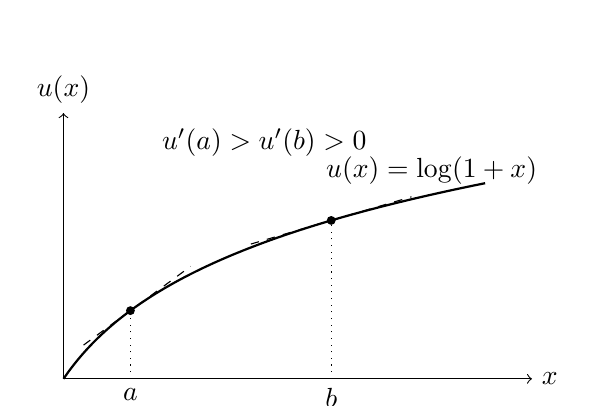
\begin{tikzpicture}[x=0.85cm,y=1.25cm]
        \draw[->] (0,0) -- (7,0) node[right] {$x$};
        \draw[->] (0,0) -- (0,2.7) node[above] {$u(x)$};
        \draw[thick,domain=0:6.3,samples=80,smooth] plot (\x,{ln(1+\x)});
        \node[above] at (5.5,{ln(6.5)}) {$u(x)=\log(1+x)$};
        \draw[dotted] (1,0) node[below] {$a$} -- (1,{ln(2)});
        \draw[dotted] (4,0) node[below] {$b$} -- (4,{ln(5)});
        \draw[dashed,domain=0.3:1.9,samples=2] plot (\x,{ln(2)+(\x-1)/2});
        \draw[dashed,domain=2.8:5.2,samples=2] plot (\x,{ln(5)+(\x-4)/5});
        \fill (1,{ln(2)}) circle (1.6pt);
        \fill (4,{ln(5)}) circle (1.6pt);
        \node at (3,2.4) {$u'(a)>u'(b)>0$};
    \end{tikzpicture}
    \end{center}

    For the unweighted sum in the question, let
    \[ F(\delta)=u(a+\delta)+u(b-\delta). \]
    When $0\leq\delta<(b-a)/2$, we have $a+\delta<b-\delta$. Since $u'$ is strictly decreasing,
    \[ F'(\delta)=u'(a+\delta)-u'(b-\delta)>0. \]
    Thus, for $0<\delta<(b-a)/2$,
    \[ F(\delta)-F(0)=\int_0^\delta F'(s)\,\mathrm{d}s>0, \]
    which gives
    \[ u(a+\delta)+u(b-\delta)>u(a)+u(b). \]

    This transfer must still be feasible. For example, starting from $(6,3)$, transferring $\delta$ units of service from user 1 to user 2 gives $(6-\delta,3+\delta)$, whose resource use is
    \[ (6-\delta)+2(3+\delta)=12+\delta>12. \]
    The transfer would violate the budget. Strict concavity therefore does not guarantee equal optimal service rates under this resource constraint.

    \subpart{(c)}
    For total service,
    \[ x_1+x_2=(x_1+2x_2)-x_2\leq12. \]
    Equality is attained only at $(x_1,x_2)=(12,0)$, so this is the optimal allocation.

    For logarithmic utility, increasing either rate increases utility, so the full budget is used. Substitute $x_1=12-2x_2$, with $0<x_2<6$, and let
    \[ f(x_2)=\log(12-2x_2)+\log x_2. \]
    Then
    \[ f'(x_2)=-\frac2{12-2x_2}+\frac1{x_2},\qquad f''(x_2)=-\frac4{(12-2x_2)^2}-\frac1{x_2^2}<0. \]
    Solving $f'(x_2)=0$ gives
    \[ 12-2x_2=2x_2,\qquad x_2=3,\qquad x_1=6. \]
    Strict concavity makes $(6,3)$ the unique maximum.

    For minimum service, let $m=\min\{x_1,x_2\}$. Since both rates are at least m,
    \[ 3m\leq x_1+2x_2\leq12,\qquad m\leq4. \]
    The allocation $(4,4)$ attains this bound and is therefore optimal.

    The results are
    \begin{center}
    \begin{tabular}{lccc}
        \toprule
        Objective & Optimal allocation & Total service & Minimum service \\
        \midrule
        Total service & $(12,0)$ & $12$ & $0$ \\
        Logarithmic utility & $(6,3)$ & $9$ & $3$ \\
        Minimum service & $(4,4)$ & $8$ & $4$ \\
        \bottomrule
    \end{tabular}
    \end{center}
    Logarithmic utility gives proportional fairness. Here it gives neither the largest total service nor equal service rates. The two users use equal amounts of resource, $x_1=2x_2=6$, even though their service rates differ.

    For the general claim, fix any $\mathbf y\in\mathcal C$. Convexity of $\mathcal C$ ensures that
    \[ \mathbf x(\theta)=\mathbf x^*+\theta(\mathbf y-\mathbf x^*)\in\mathcal C,\qquad0\leq\theta\leq1. \]
    Set
    \[ h(\theta)=\sum_{i=1}^n\log\bigl(x_i^*+\theta(y_i-x_i^*)\bigr). \]
    Since $\mathbf x^*$ is optimal, $h(\theta)\leq h(0)$ for $\theta\geq0$ in this interval. Taking the right derivative at zero gives
    \[ h'(0^+)=\sum_{i=1}^n\frac{y_i-x_i^*}{x_i^*}\leq0. \]
    Each term is a user's change in service relative to the original service rate. Thus no feasible change has a positive sum of proportional changes: the proportional gains cannot exceed the proportional losses. This is the proportional-fairness condition.

    With the weighted objective $2\log x_1+\log x_2$, the full budget is again used. Let
    \[ g(x_2)=2\log(12-2x_2)+\log x_2. \]
    Then
    \[ g'(x_2)=-\frac4{12-2x_2}+\frac1{x_2},\qquad g''(x_2)=-\frac8{(12-2x_2)^2}-\frac1{x_2^2}<0. \]
    Setting $g'(x_2)=0$ gives
    \[ 12-2x_2=4x_2,\qquad x_2=2,\qquad x_1=8. \]
    Hence the optimal allocation is $(8,2)$. The coefficient 2 is user 1's utility weight: the same small percentage increase in service contributes twice as much to the objective for user 1 as for user 2. This gives weighted proportional fairness. This weight and the resource cost 2 in the constraint describe different things.

    \subpart{(d)}
    Under the expected-payoff objective, the options are tied:
    \[ \E[X_A]=5,\qquad \E[X_B]=\frac12\cdot1+\frac12\cdot9=5. \]
    Under expected logarithmic utility,
    \[ \E[\log X_A]=\log5,\qquad \E[\log X_B]=\frac12\log1+\frac12\log9=\log3. \]
    Since $\log5>\log3$, option A is preferred. The certainty equivalent c of option B satisfies
    \[ \log c=\log3,\qquad c=3. \]

    For a concave utility function, Jensen's inequality gives
    \[ \E[u(X)]\leq u(\E[X]). \]
    Thus the certain payoff $\E[X]$ is at least as good as the lottery under expected utility. If u is strictly concave and the lottery is nonconstant, the preference is strict. This is risk aversion.

    Here the expectation averages uncertain outcomes for one user. In part (b), the sum combines deterministic service rates for different users. Concavity gives risk aversion in the first setting and favors more balanced service in the second, subject to feasibility.

    \subpart{(e)}
    For lotteries over a finite set of outcomes $\{z_1,\ldots,z_m\}$, the four preference axioms are:
    \begin{enumerate}
        \item \textbf{Completeness.} For any lotteries L and M, $L\succeq M$ or $M\succeq L$, or both.
        \item \textbf{Transitivity.} If $L\succeq M$ and $M\succeq N$, then $L\succeq N$.
        \item \textbf{Continuity.} If $L\succ M\succ N$, some $\alpha\in(0,1)$ satisfies
        \[ M\sim\alpha L+(1-\alpha)N. \]
        \item \textbf{Independence.} For any lottery N and $\alpha\in(0,1)$,
        \[ L\succeq M\quad\Longleftrightarrow\quad\alpha L+(1-\alpha)N\succeq\alpha M+(1-\alpha)N. \]
        Mixing both options with the same lottery in the same proportions preserves their ranking.
    \end{enumerate}

    The von Neumann--Morgenstern theorem states that these axioms are equivalent to an expected-utility representation. There is a utility u on outcomes such that, if L assigns probabilities $p_j$ and M assigns probabilities $q_j$,
    \[ L\succeq M\quad\Longleftrightarrow\quad\sum_{j=1}^m p_j u(z_j)\geq\sum_{j=1}^m q_j u(z_j). \]
    The utility is unique up to a positive affine transformation:
    \[ \widetilde u(z)=A u(z)+B,\qquad A>0. \]
    Such a transformation preserves the ranking because $\E[\widetilde u(X)]=A\E[u(X)]+B$.

    The theorem does not require concave or logarithmic utility. It describes one decision maker's preferences over lotteries, so it does not choose a fairness criterion or utility weights across users.

    A strictly increasing transformation preserves the ranking of deterministic outcomes, but it can change the ranking of expected utilities. In part (d), $u(x)=x$ makes A and B equally good because both have mean 5. The transformation $v(x)=\log u(x)=\log x$ preserves the ordering of positive payoffs, but now $\log5>\log3$, so A is strictly preferred. Thus the same ranking of certain outcomes can lead to different choices under uncertainty.

    \subpart{(f)}
    The reward hypothesis proposes that goals can be expressed by maximizing the expected cumulative sum of scalar rewards. In this undiscounted finite episode, this means maximizing
    \[ J(\pi)=\E_\pi\left[\sum_{t=0}^{T-1}R_{t+1}\right]. \]
    If an episode's utility is its total reward, this is expected-utility maximization. However, the expected utility theorem alone does not produce a stationary Markov reward on a prescribed state space. The utility may depend on past events that the current state does not record.

    For $T=2$, all allocations in the two schedules are positive and use the full budget. The instantaneous-utility values are
    \[
    \begin{aligned}
        J_{\mathrm{instant}}(\pi_A)
        &=2(\log6+\log3)=2\log18=\log324,\\
        J_{\mathrm{instant}}(\pi_B)
        &=\log10+\log1+\log2+\log5=\log100.
    \end{aligned}
    \]
    Thus the instantaneous objective prefers $\pi_A$.

    The time averages are
    \[ (\overline X_1,\overline X_2)_{\pi_A}=(6,3),\qquad (\overline X_1,\overline X_2)_{\pi_B}=\left(\frac{10+2}{2},\frac{1+5}{2}\right)=(6,3). \]
    Hence
    \[ J_{\mathrm{average}}(\pi_A)=J_{\mathrm{average}}(\pi_B)=\log18. \]
    The two objectives are not equivalent: one strictly prefers $\pi_A$, while the other treats the schedules equally. The first evaluates service at each time step; the second uses only the average service over the episode.

    To construct rewards for $J_{\mathrm{average}}$, keep track of cumulative service:
    \[ C_i(0)=0,\qquad C_i(t+1)=C_i(t)+X_i(t),\qquad i=1,2. \]
    Give zero reward until the last transition, and then give
    \[
    R_{t+1}=\begin{cases}
        0,&0\leq t<T-1,\\[3pt]
        \displaystyle\log\frac{C_1(T)}T+\log\frac{C_2(T)}T,&t=T-1.
    \end{cases}
    \]
    Since $C_i(T)/T=\overline X_i$, every episode satisfies
    \[ \sum_{t=0}^{T-1}R_{t+1}=\log\overline X_1+\log\overline X_2. \]
    Taking expectations gives
    \[ \E_\pi\left[\sum_{t=0}^{T-1}R_{t+1}\right]=J_{\mathrm{average}}(\pi). \]

    If these quantities are not already in the state, use
    \[ \widetilde s_t=(s_t,t,C_1(t),C_2(t)). \]
    The cumulative totals record the service so far, and t identifies the last step. For fixed T, the reward can then be computed from the augmented state and next state using the same rule at every transition.

    \subpart{(g)}
    A policy induces a probability distribution over episode outcomes. In the finite-outcome setting of part (e), if preferences over lotteries on these outcomes satisfy the four axioms, there is a utility U such that policies are compared by
    \[ \E_\pi[U(\tau)], \]
    where $\tau$ denotes a complete trajectory. If rewards are chosen so that
    \[ U(\tau)=\sum_{t=0}^{T-1}R_{t+1}, \]
    then
    \[ \E_\pi[U(\tau)]=\E_\pi\left[\sum_{t=0}^{T-1}R_{t+1}\right]=J(\pi). \]
    This connects expected-utility maximization with the reward hypothesis. The additional step is to choose a utility and construct rewards that represent it. The theorem does not specify the fairness objective or guarantee a Markov reward on the original state space. Part (f) shows how adding cumulative service and time to the state can supply the information needed by a history-dependent objective.

\end{homeworkProblem}

\end{document}
